\begin{center}
    \begin{tikzpicture}[
        node/.style={
            circle, 
            draw,
            radius=1cm,
        },
        head/.style={
            rectangle, 
            draw,
            minimum width=2cm,
            minimum height=1cm,
        },
    ]

    \node (C1) at (0,0) [node] {C1};
    \node (C2) at (2,0) [node] {C2};    

    \draw [->] (C2) -- (C1);
    
    \only<1>{
        \node (h1) at (2, -2) [head] {HEAD};
        \draw [->] (h1) -- (C2);
    }

    \pause
    \node (C3) at (4,0) [node] {C3};
    \draw [->] (C3) -- (C2);
    
    \only<2>{
        \node (h2) at (4, -2) [head] {HEAD};
        \draw [->] (h2) -- (C3);
    }
    \pause

    \node (C4) at (6,0) [node] {C4};
    \draw [->] (C4) -- (C3);

    \only<3>{
        \node (h3) at (6, -2) [head] {HEAD};
        \draw [->] (h3) -- (C4);
    }
    
    \onslide<1->
    \end{tikzpicture}
\end{center}